%%%%%%%%%%%%%%%%%%%%%%%%%%%%%%%%%%%%%%%%%%  不使用 authblk 包制作标题  %%%%%%%%%%%%%%%%%%%%%%%%%%%%%%%%%%%%%%%%%%%%%%
%-------------------------------PPT Title-------------------------------------
\title{17-旋-轨耦合相互作用的本质}
%-----------------------------------------------------------------------------
%----------------------------Author & Date------------------------------------

%\author[\textrm{Jun\_Jiang}]{姜\;\;骏\inst{}} %[]{} (optional, use only with lots of authors)
%% - Give the names in the same order as the appear in the paper.
%% - Use the \inst{?} command only if the authors have different
%%   affiliation.
%\institute[BCC]{\inst{}%
\institute[Gain~Strong]{\inst{}%
%\vskip -20pt 北京市计算中心}
\vskip -20pt {\large 格致斯创~科技}}
\date[\today] % (optional, should be abbreviation of conference name)
{%	{\fontsize{6.2pt}{4.2pt}\selectfont{\textcolor{blue}{E-mail:~}\url{jiangjun@bcc.ac.cn}}}
\vskip 45 pt {\fontsize{8.2pt}{6.2pt}\selectfont{%清华大学\;\;物理系% 报告地点
	\vskip 5 pt \textrm{2023.07.29}}}
}

%% - Either use conference name or its abbreviation
%% - Not really information to the audience, more for people (including
%%   yourself) who are reading the slides onlin%%   yourself) who are reading the slides onlin%%   yourself) who are reading the slides onlineee
%%%%%%%%%%%%%%%%%%%%%%%%%%%%%%%%%%%%%%%%%%%%%%%%%%%%%%%%%%%%%%%%%%%%%%%%%%%%%%%%%%%%%%%%%%%%%%%%%%%%%%%%%%%%%%%%%%%%%

\subject{}
% This is only inserted into the PDF information catalog. Can be left
% out.
%\maketitle
\frame
{
%	\frametitle{\fontsize{9.5pt}{5.2pt}\selectfont{\textcolor{orange}{“高通量并发式材料计算算法与软件”年度检查}}}
\titlepage
}
%-----------------------------------------------------------------------------

%------------------------------------------------------------------------------列出全文 outline ---------------------------------------------------------------------------------
%\section*{}
%\frame[allowframebreaks]
%{
%  \frametitle{Outline}
%%  \frametitle{\textcolor{mycolor}{\secname}}
%  \tableofcontents%[current,currentsection,currentsubsection]
%}
%%在每个section之前列出全部Outline
%%类似的在每个subsection之前列出全部Outline是\AtBeginSubsection[]
%\AtBeginSection[]
%{
%  \frame<handout:0>%[allowframebreaks]
%  {
%    \frametitle{Outline}
%%全部Outline中,本部分加亮
%    \tableofcontents[current,currentsection]
%  }
%}

%-----------------------------------------------PPT main Body------------------------------------------------------------------------------------
\small
%\section{\rm{VASP~}软件中\rm{PAW~}计算的实现}
%\frame
%
%	\frametitle{\textrm{VASP}计算的特色}
%	相比于与普通的第一原理计算软件,\textrm{VASP}很好地平衡了计算效率和精度的问题,总的来说,\textrm{VASP}主要通过这几个特色保证了计算的高效能
%	\begin{itemize}
%	     \item 迭代与优化算法的多样性\\
%		     本质上电荷密度迭代 \textrm{\&\&} 体系总能量优化是相同的优化问题,采用了类似的算法\upcite{CMS6-15_1996,PRB54-11169_1996}:\\
%			\textcolor{blue}{\textrm{Pseudo-Newton、Conjugate-Gradient、Broyden~mix、damping-factor、RMM-DIIS}}
%	     \item 尽可能采用局域基(原子轨道基)函数:~\\
%		     \textcolor{blue}{\textrm{LREAL}}=\textcolor{red}{\textrm{.TRUE.}}\\
%			优化的投影函数也尽可能在实空间表示
%	     \item \textrm{PAW}原子数据集:\textcolor{blue}{优异的赝势}\upcite{PRB59-1758_1999}
%	\end{itemize}
%}
\section{旋-轨耦合作用的本质}
\frame
{
\frametitle{旋-轨耦合的起源}
\begin{figure}[h!]
\centering
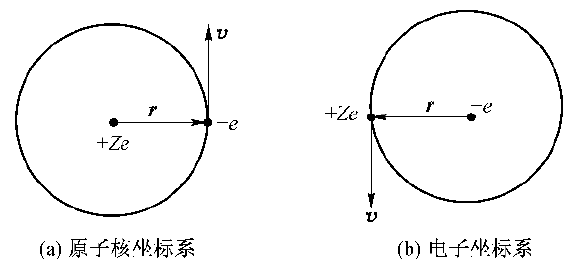
\includegraphics[height=1.75in,width=3.95in,viewport=0 0 600 270,clip]{Figures/SOC_cor.png}
\caption{\tiny \textrm{A schematic coordinate for an electron in atom: (a) atomic coordinate system, (b) electron coordinate ones.}}%(与文献\cite{EPJB33-47_2003}图1对比)
\label{Nuclear_Electron}
\end{figure}
自旋-轨道耦合本质:~\textcolor{red}{外电场对运动自旋磁矩的作用,是相对论效应}
}

\frame
{
\frametitle{核-电子运动与电-磁场}
\begin{itemize}
	\item 静止电荷间的静电力作用(\textrm{Coulomb}力)
		\begin{displaymath}
			\begin{aligned}
				\vec F_1=&\dfrac{q_1q_2}{4\pi\epsilon_0}\dfrac{\hat r_{12}}{|\vec r_{12}|^2}\\
				\vec F_2=-\vec F_1
			\end{aligned}
		\end{displaymath}
	\item 电场对运动的电荷的作用
		\begin{displaymath}
			\vec F=q\vec E
		\end{displaymath}
	\item 磁场对运动的电荷力的作用(\textrm{Lorentz}力)
		\begin{displaymath}
		\vec F=q\vec v\times\vec B
		\end{displaymath}
\end{itemize}
}

\frame
{
	\frametitle{经典唯象的旋-轨耦合}
	\begin{itemize}
		\item 在原子核坐标系下,根据\textrm{Coulomb}定理,运动电子$-e$的速度为$v$~,并存在自旋磁矩,离子实会与运动电子的磁矩发生相互作用
		\item 由于运动是相对的,在电子坐标系下,旋-轨耦合可理解为电场$\vec E$以速度$-v$运动产生磁场$\vec B$,磁场会对电子自旋有力的作用
	\end{itemize}
	\begin{displaymath}
		\vec B=\frac{\mu_0\vec j\times\vec r}{r^3}=\mu_0\varepsilon_0(\vec v\times\vec E)
	\end{displaymath}
其中$\vec v$是电子运动速度,$\vec E$是离子实在电子处的电场。根据电场强度的径向分布形式
\begin{displaymath}
	\vec E=\frac1{e}\frac{\partial V}{\partial r}\frac{\vec r}r
\end{displaymath}
利用轨道角动量关系$\vec L=\vec r\times\vec p$和$\vec p=m\vec v$,可得磁感应强度
\begin{displaymath}
	\vec B=\frac1{emc^2}\frac1r\frac{\partial V}{\partial r}\vec L
\end{displaymath}
}

\frame
{
	\frametitle{经典唯象的旋-轨耦合}
对自由电子自旋,离子实在电子处的磁场对\textrm{Hamiltonian}贡献为
\begin{displaymath}
	\vec H=\frac{(\vec{\sigma}\cdot\vec p)^2}{2m}
\end{displaymath}

考虑磁场与交变电磁场$\mathbf{A}$:~$\mathbf B=\nabla\times\mathbf A$,因此
\begin{displaymath}
	H=\frac{\left( \vec{\sigma}\cdot\left( \vec p+\dfrac ec\mathbf A \right) \right)^2}{2m}
\end{displaymath}
利用关系式$(\vec{\sigma}\cdot\mathbf A)(\vec{\sigma}\cdot\mathbf B)=\mathbf{A}\cdot\mathbf{B}+\mathrm{i}\vec{\sigma}(\mathbf{A}\times\mathbf{B})$,可得
\begin{displaymath}
	H=\frac{\left( \vec p+\frac ec\mathbf{A} \right)^2}{2m}+\underline{\textcolor{red}{\frac{\mathrm i}{2m}\vec{\sigma}\cdot\left( \vec p+\frac ec\mathbf{A} \right)\times\left( \vec p+\frac ec\mathbf{A} \right)}}
\end{displaymath}
其中第一项是轨道磁矩与外磁场相互作用,第二项是自旋磁矩与外磁场相互作用
}

\frame
{
	\frametitle{经典唯象的旋-轨耦合}
	自旋磁矩与外场相互作用
	\begin{displaymath}
		\begin{aligned}
			&\frac{\mathrm{i}e}{2mc}\vec\sigma\cdot[(\vec p\times\mathbf{A})+(\mathbf{A}\times\vec p)]=\frac{\mathrm{i}e}{2mc}\vec{\sigma}\cdot(-\mathrm{i}\hbar\nabla\times\mathbf{A})\\
			=&\frac{e\hbar}{2mc}\vec{\sigma}\cdot\mathbf{B}=-\vec{\mu}_s\cdot\mathbf{B}
		\end{aligned}
	\end{displaymath}
	其中$\vec \mu_s=-g_s\mu_B\vec S$,是电子自旋$\vec S$磁矩,$g_s$是电子自旋$g$因子,$\mu_B$是\textrm{Bohr}磁子,$\vec S$是自旋角动量,因此可得自旋-轨道相互作用能量为:
	\begin{displaymath}
		\begin{aligned}
			U=&\frac1{m^2c^2}\frac1r\frac{\partial V}{\partial r}\vec L\cdot\vec S\\
			=&-\frac1{m^2c^2}\nabla V\cdot(\vec S\times\vec p)
		\end{aligned}
	\end{displaymath}
	由于电子的高速运动,考虑电子参照系的非惯性系性质,会产生\textrm{Thomas}进动,因此非惯性系中真空自旋-轨道耦合\textrm{Hamiltonian}为
	\begin{displaymath}
		\vec H_{\mathrm{SO}}=-\frac1{4m^2c^2}(\vec S\cdot\vec p)\times\nabla V
	\end{displaymath}
}

\frame
{
	\frametitle{类\textrm{H}原子旋-轨耦合的估计}
\begin{minipage}{0.58\textwidth}
	\begin{displaymath}
		\begin{aligned}
			V(r)=&-\dfrac1{4\pi\epsilon_0}\dfrac{Ze^2}r~\quad(\mbox{\textrm{Z}是核电荷数})\\
			E_n=&-\dfrac{\mu c^2Z^2\alpha^2}{2n^2}\\
			r_1\approx&\bigg(\dfrac{4\pi\epsilon_0}{e^2}\bigg)\dfrac{\hbar^2}{Zm_e} ~~ \sim Z^{-1}\\
			v_1=&\dfrac{Ze^2}{4\pi\epsilon_0\hbar}\sim Z\\
			mv^2=&\dfrac{Ze^2}{4\pi\epsilon_0r_n}~~\sim Z^2\\
			E=&\nabla V(r)=\dfrac1{4\pi}\dfrac{Ze^2}{r^2}\hat r ~~ \sim Z^3
		\end{aligned}
	\end{displaymath}
\end{minipage}
\begin{minipage}{0.40\textwidth}
\begin{figure}[h!]
\centering
\vspace{-0.9in}
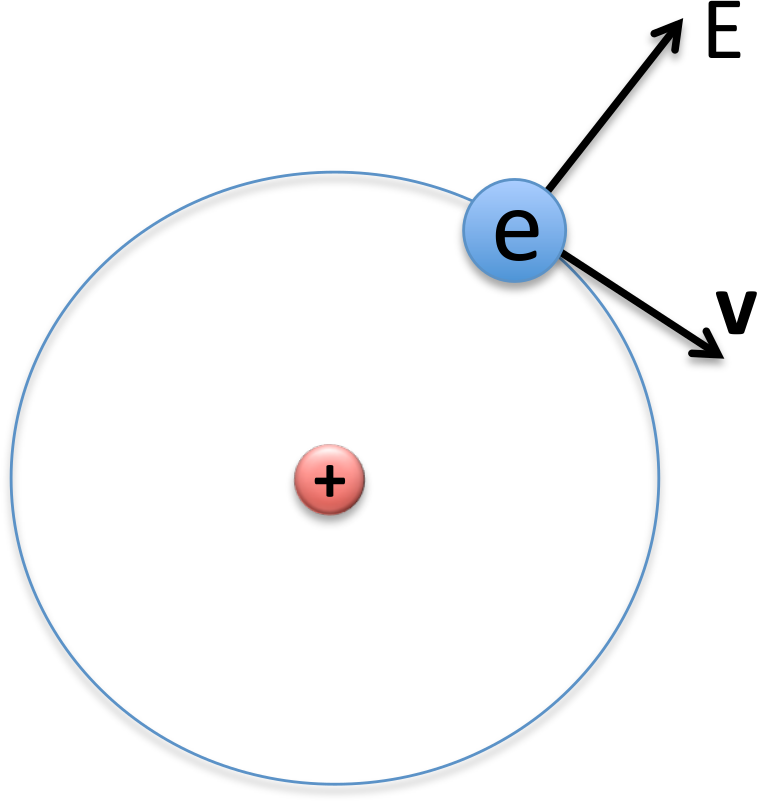
\includegraphics[height=1.35in,width=1.3in,viewport=0 0 760 800,clip]{Figures/SOC_hydrogen-H_atom.png}
%\caption{\textrm{The wave-particle duality and Photoelectric effect}}
\label{SOC-hydrongen-like-1}
\end{figure}
\end{minipage}
}

\frame
{
	\frametitle{类\textrm{H}原子旋-轨耦合的估计}
\begin{minipage}{0.58\textwidth}
	\begin{itemize}
		\item 电子自旋产生的电子磁矩\textrm{(in~SI)}
			\begin{displaymath}
				\vec\mu_s=-\dfrac{e}{m}\vec S=-\dfrac{e}{m}\dfrac{h}2\vec\sigma=-\mu_b\vec\sigma=-\dfrac{2\mu_B}{\hbar}\vec S
			\end{displaymath}
		\item 轨道角动量形成的轨道磁矩
			\begin{displaymath}
				\vec\mu_L=-\dfrac{e}{2m}\vec L=-\dfrac{\mu_B}{\hbar}\vec L=-\mu_B\vec l
			\end{displaymath}
			可以理解为电子的轨道运动形成的电流,产生的磁场$\vec H_{\mathrm{eff}}$
		\item 自旋-轨道相互作用的静态能量
			\begin{displaymath}
				E_{\mathrm{SO}}=-\vec\mu_s\cdot\mathbf{B}_{\mathrm{eff}}
			\end{displaymath}
			也就是\textcolor{blue}{静电-磁偶极相互作用}
	\end{itemize}
\end{minipage}
\begin{minipage}{0.40\textwidth}
\begin{figure}[h!]
\centering
\vspace{+0.3in}
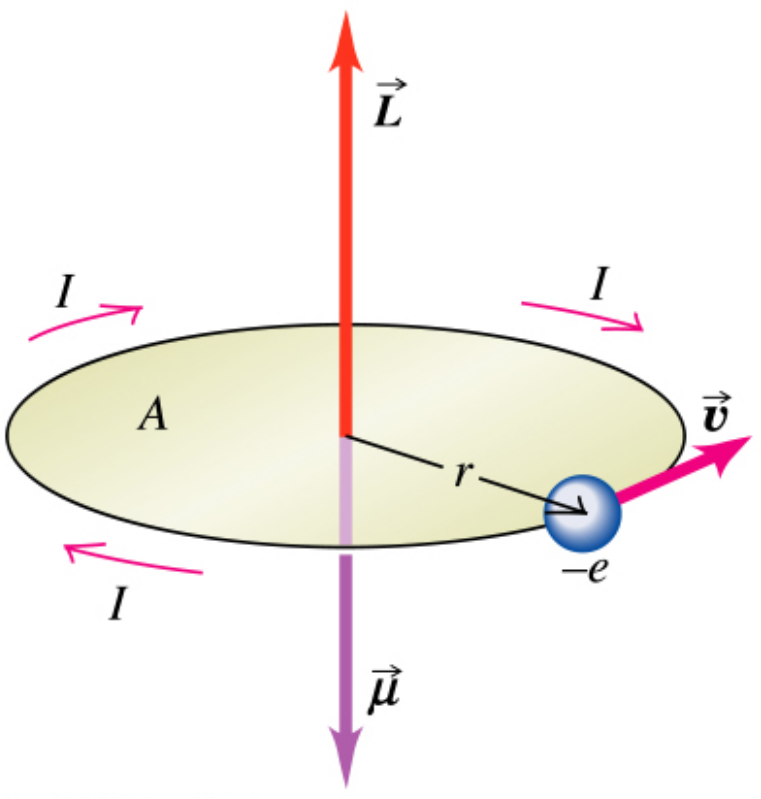
\includegraphics[height=1.55in,width=1.38in,viewport=0 0 760 800,clip]{Figures/SOC_spin-orbit.png}
%\caption{\textrm{The wave-particle duality and Photoelectric effect}}
\label{SOC_spin-orbit}
\end{figure}
\end{minipage}
}

\frame
{
	\frametitle{类\textrm{H}原子旋-轨耦合的估计}
\begin{minipage}{0.58\textwidth}
	\begin{displaymath}
		\begin{aligned}
			E_n=&-\dfrac{\mu c^2Z^2\alpha^2}{2n^2}~\sim -13.6\bigg(\dfrac{Z^2}{n^2}\bigg)\mathrm{eV}\\
			r_1\approx&\bigg(\dfrac{4\pi\epsilon_0}{e^2}\bigg)\dfrac{\hbar^2}{Zm_e} ~~ a_0=0.529Z^{-1}\AA\\
			v_1=&\dfrac{Ze^2}{4\pi\epsilon_0\hbar}\sim \dfrac{Z}{137}c\\
			\gamma\equiv&\dfrac1{\sqrt{1-v^2/c^2}}~\quad \mbox{\textrm{Lorentz~factor\quad(\textcolor{blue}{Relativistic~effect})}}\\
			m=&\gamma m_0=m_0/\sqrt{1-(v/c)^2}\\
			a_0=&\hbar^2/me^2
		\end{aligned}
	\end{displaymath}
\end{minipage}
\begin{minipage}{0.40\textwidth}
\begin{figure}[h!]
\centering
\vspace{-0.9in}
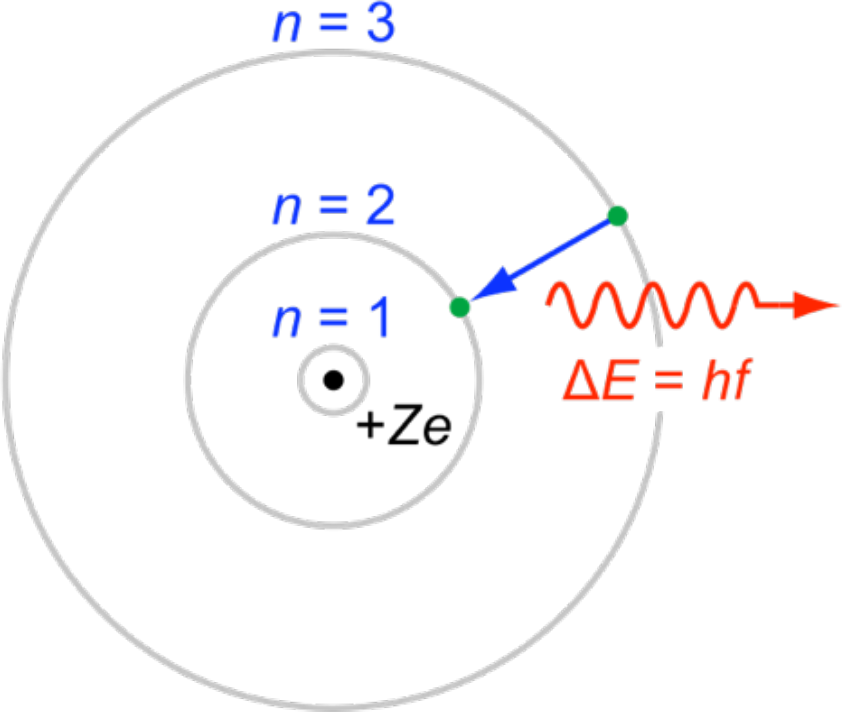
\includegraphics[height=1.35in,width=1.38in,viewport=0 0 840 800,clip]{Figures/SOC_hydrogen-H_electron.png}
%\caption{\textrm{The wave-particle duality and Photoelectric effect}}
\label{SOC-hydrongen-like-2}
\end{figure}
\end{minipage}
}

\frame
{
	\frametitle{类\textrm{H}原子旋-轨耦合的估计}
	\begin{itemize}
		\item \textrm{Lorentz~transformation}
			\begin{displaymath}
				\begin{aligned}
					\mathbf{E}_{\parallel}^{\prime}=&\mathbf{E}_{\parallel}\qquad\qquad \mathbf{B}_{\parallel}^{\prime}=\mathbf{B}_{\parallel}\\
					\mathbf{E}_{\perp}^{\prime}=&\gamma(\mathbf{E}_{\perp}+\vec v\times\mathbf{B})\\
					\mathbf{B}_{\perp}^{\prime}=&\gamma\bigg(\mathbf{B}_{\perp}-\dfrac1{c^2}\vec v\times\mathbf{E}\bigg)
				\end{aligned}
			\end{displaymath}
	\end{itemize}
	这里
	\begin{displaymath}
		\begin{aligned}
			\mathbf{B}=&\dfrac1{c^2}\mathbf{E}\times\vec v~\sim Z^4\\
			\mathbf{E}=&-\dfrac{\vec r}r\phi^{\prime}\qquad\qquad \mathbf{B}=-\dfrac1{rc^2}\phi^{\prime}\vec r\times\vec v
		\end{aligned}
	\end{displaymath}
	注意到$\vec l=\vec r\times\vec p$,因此有$\vec r\times\vec v=\dfrac1{m_e}\vec l$,因此有\textrm{Hamiltonian}
	\begin{displaymath}
		h_{\mathrm{SO}}=-\mu_{e}\cdot\mathbf{B}=\dfrac1{m_erc^2}\phi^{\prime}\mu\cdot\vec l=\dfrac{e}{m_e^2c^2}\dfrac{\phi^{\prime}}r\vec\sigma\cdot\vec l \quad\textcolor{blue}{\Longleftarrow\mbox{\textrm{\fontsize{6.5pt}{5.2pt}\selectfont{1/2~Thomas~factor}}}}
	\end{displaymath}
}

\frame
{
	\frametitle{\textrm{Dirac~}方程}
	自旋是相对论量子力学的自然结果,严格地给出自旋-轨道耦合必须要从\textrm{Dirac~}方程出发,由\textrm{Dirac~}方程的非相对论极限可得到旋-轨耦合的具体形式,由\textrm{Dirac~}算符
	\begin{displaymath}
		\vec H_{\mathrm D}=c\vec{\alpha}\cdot\vec p+(\vec{\beta}-1)mc^2+V(\vec r)
	\end{displaymath}
	其中$\mathbf{\alpha}$和$\mathbf{\beta}$是$4\times4$的矩阵
	\begin{displaymath}
		\vec{\alpha}=\left(
		\begin{matrix}
			0 &\vec{\sigma}\\
			\vec{\sigma} &0
		\end{matrix}
		\right)\quad\beta=\left(
		\begin{matrix}
			1 &0 &0 &0\\
			0 &1 &0 &0\\
			0 &0 &-1 &0\\
			0 &0 &0 &-1
		\end{matrix}
		\right)
	\end{displaymath}
	$\vec{\sigma}$是\textrm{Pauli-spin~}矩阵,
	\begin{displaymath}
		\sigma_x=\left( 
		\begin{matrix}
			0 &1\\
			1 &0
		\end{matrix}
		\right)\quad
		\sigma_y=\left( 
		\begin{matrix}
			0 &-\mathrm{i}\\
			\mathrm{i} &0
		\end{matrix}
		\right)\quad
		\sigma_z=\left( 
		\begin{matrix}
			1 &0\\
			0 &-1
		\end{matrix}
		\right)
	\end{displaymath}
	$p=-\mathrm{i}\nabla$是动量算符,$c$是光速(原子单位下$c=274.0746$)
}

\frame
{
	\frametitle{二分量\textrm{Dirac~}方程}
	在低速非相对论近似下,可以把正负能态间的耦合作为微扰处理,可以得到二分量方程(\textrm{Pauli~}方程),其解是四分量波函数$\Psi$,可以写成二分量函数形式$\Phi$、$\chi$
	\begin{displaymath}
		\Psi=\left( 
		\begin{matrix}
			\Phi\\
			\chi
		\end{matrix}
		\right)
	\end{displaymath}
	$\Phi$称为波函数的\textcolor{blue}{大分量部分},$\chi$称为波函数的\textcolor{blue}{小分量部分}

	$\Phi$和$\chi$是耦合方程:%,在没有外场$\mathbf{A}$时
	\begin{displaymath}
		\begin{aligned}
			c(\vec{\sigma}\cdot\vec p)\chi&=(\varepsilon-V)\Phi\\
			c(\vec{\sigma}\cdot\vec p)\Phi&=(\varepsilon-V+2mc^2)\chi
		\end{aligned}
	\end{displaymath}
	由此得到大分量组分方程
	\begin{displaymath}
		\frac1{2m}(\vec{\sigma}\cdot\vec p)\left( 1+\frac{\varepsilon-V}{2mc^2} \right)^{-1}(\vec{\sigma}\cdot\vec p)\Phi+V\Phi=\varepsilon\Phi	
	\end{displaymath}
}

\frame
{
	\frametitle{二分量\textrm{Dirac~}方程}
	利用近似$$\left( 1+\frac{\varepsilon-V}{2mc^2} \right)^{-1}\approx1-\frac{\varepsilon-V}{2mc^2}$$
	并有
	\begin{displaymath}
		\begin{aligned}
			\vec pV&=V\vec p-\mathrm{i}\hbar\nabla V\\
			(\vec{\sigma}\nabla V)(\vec{\sigma}\cdot\vec p)&=(\nabla V\vec p)+\mathrm{i}\vec{\sigma}[\nabla,\vec p]
		\end{aligned}
	\end{displaymath}
	由此得$\Phi$的微分方程
	\begin{displaymath}
		\hspace*{-10pt}	\left[ \left( 1-\frac{\varepsilon-V}{2mc^2} \right)\frac{\vec p^2}{2m}+V \right]\Phi-\frac{h^2}{4m^2c^2}(\nabla V\nabla \Phi)+\frac{h^2}{4m^2c^2}(\sigma[\nabla V,\vec p]\Phi)=\varepsilon\Phi
	\end{displaymath}
}

\frame
{
	\frametitle{中心力场的\textrm{Dirac~}方程}
	在球形对称势函数条件下
	\fontsize{9.5pt}{5.2pt}\selectfont{\begin{displaymath}
		\hspace*{-10pt}\left[ \underline{\textcolor{blue}{\frac{p^2}{2m}+V}}-\textcolor{brown}{\dfrac{\hbar}{2m}\vec{\sigma}\cdot\vec B}-\textcolor{magenta}{\frac{p^4}{8m^3c^2}}-\textcolor{magenta}{\frac{\hbar^2}{4m^2c^2}\frac{\mathrm{d}V}{\mathrm{d}r}\frac{\partial}{\partial\vec r}}+\underline{\textcolor{red}{\frac1{2m^2c^2}\frac1r\frac{\mathrm{d}V}{\mathrm{d}r}(\vec l\cdot\vec\sigma)}} \right]\Phi=\varepsilon\Phi
	\end{displaymath}}
	\begin{itemize}
		\item 第一与第二项是非相对论\textrm{Schr\"odinger~}方程
		\item 第三项是自旋与磁场的相互作用:~\textrm{Zeeman}项
		\item 第四和第五项是相对论效应的质量校正和\textrm{Darwin~}校正
		\item 最后一项对应于自旋-轨道耦合
	\end{itemize}
	考虑旋-轨耦合后,波函数$\Psi$不再是自旋或轨道角动量的本征态,新的好量子数$j$、$j_z$和$\kappa$定义为
	$$\begin{aligned}
		\vec j&=\vec l+\vec s\\
%		\vec j_z&=\vec l_z+\vec s_z
	\end{aligned}$$
	$\hbar\kappa$是算符
	\begin{displaymath}
		K=\left( 
		\begin{matrix}
			\vec{\sigma}\cdot\vec l+\hbar &0\\
			0 &-\vec{\sigma}\cdot\vec l-\hbar
		\end{matrix}
		\right)
	\end{displaymath}
	的本征值
%	
%	$\kappa$和$j$的关系是
%	$$\kappa=\pm(j+\frac12)$$
}

\frame
{
	\frametitle{中心力场的\textrm{Dirac~}方程}
	球对称下的\textrm{Dirac~}方程解,二分量波函数$\Psi$因此可写成
	\begin{displaymath}
		\Psi=\left( 
		\begin{matrix}
			\Phi\\
			\chi
		\end{matrix}
		\right)=\left( 
		\begin{matrix}
			g_{\kappa}(r)\mathcal{Y}_{jl}^{j_z}\\
			\mathrm{i}f_{\kappa}(r)\mathcal{Y}_{jl^{\prime}}^{j_z}
		\end{matrix}
		\right)
	\end{displaymath}
	$g$和$f$是径向函数,相对论量子数$\kappa$满足$\kappa=\pm(j+\frac12)$,$\mathcal{Y}_{jl}^{j_z}$是二分量自旋-角动量本征态函数,满足
	\begin{displaymath}
		\begin{aligned}
			-(1+\vec{\sigma}\cdot\vec l)\mathcal{Y}_{jl}^{j_z}=\kappa\mathcal{Y}_{jl}^{j_z}\\
			\vec{\sigma}\cdot\frac{\vec r}r\mathcal{Y}_{jl}^{j_z}=-\mathcal{Y}_{jl}^{j_z}
		\end{aligned}
	\end{displaymath}
	径向函数$g_{\kappa}(r)$和小分量$f_{\kappa}(r)$满足线性\textrm{Dirac~}方程
	\begin{displaymath}
		\begin{aligned}
			\left( \frac{\mathrm{d}}{\mathrm{d}r}+\frac1r-\frac{\kappa}r \right)cf_{\kappa}(r)+[\varepsilon-V(r)]g_{\kappa}(r)=0\\
			\left( \frac{\mathrm{d}}{\mathrm{d}r}+\frac1r+\frac{\kappa}r \right)g_{\kappa}(r)-\left[ 1+\frac{\varepsilon-V(r)}{c^2} \right]cf_{\kappa}(r)=0
		\end{aligned}
	\end{displaymath}
}

\frame
{
	\frametitle{中心力场的\textrm{Dirac~}方程}
	消去$f_{\kappa}(r)$,有
	\begin{displaymath}
		\begin{aligned}
			&-\frac{\hbar^2}{2Mr^2}\frac{\mathrm{d}}{\mathrm{d}r}\left[ r^2\frac{\mathrm{d}g_{\kappa}(r)}{\mathrm{d}r} \right]+\left[ V(r)+\frac{\hbar^2}{2Mr^2}\frac{l(l+1)}{r^2} \right]g_{\kappa}(r)\\
			&-\frac{\hbar^2}{4M^2c^2}\frac{\mathrm{d}V(r)}{\mathrm{d}r}\frac{\mathrm{d}g_{\kappa}(r)}{\mathrm{d}r}-\frac{\hbar^2}{4M^2c^2}\frac{\mathrm{d}V(r)}{\mathrm{d}r}\frac{1+\kappa}rg_{\kappa}(r)=\varepsilon g_{\kappa}(r)
		\end{aligned}
	\end{displaymath}
	这里引入相对论质量$$M=\dfrac{m}{\sqrt{1-\dfrac{\varepsilon-V(\mathbf{r})}{2mc^2}}}=m+\frac{\varepsilon-V(r)}{2c^2}$$
	利用等式关系$$\kappa(\kappa+1)=l(l+1)$$
	小分量$f_{\kappa}(r)$可以表示为
	\begin{displaymath}
		f_{\kappa}(r)=\frac{\hbar}{2Mc}\left( \frac{\mathrm{d}g_{\kappa}(r)}{\mathrm{d}r}+\frac{1+\kappa}rg_{\kappa}(r) \right)
	\end{displaymath}
}

\frame
{
	\frametitle{标量相对论近似}
	\textcolor{blue}{在$g_{\kappa}(r)$和$f_{\kappa}(r)$方程中}\textcolor{red}{略去有关$\kappa$项}\textcolor{blue}{即可得标量相对论方程}
	\begin{displaymath}
		\begin{aligned}
			&-\frac{\hbar^2}{2Mr^2}\frac{\mathrm{d}}{\mathrm{d}r}\left[ r^2\frac{\mathrm{d}\tilde{g}(r)}{\mathrm{d}r} \right]+\left[ V(r)+\frac{\hbar^2}{2Mr^2}\frac{l(l+1)}{r^2} \right]\tilde{g}(r)\\
			&-\frac{\hbar^2}{4M^2c^2}\frac{\mathrm{d}V(r)}{\mathrm{d}r}\frac{\mathrm{d}\tilde{g}(r)}{\mathrm{d}r}=\varepsilon\tilde{g}(r)
		\end{aligned}
	\end{displaymath}
	这里$\tilde g(r)$和$\tilde f(r)$是$g_{\kappa}(r)$和$f_{\kappa}(r)$的标量相对论近似,满足
	\begin{displaymath}
		\begin{aligned}
			&\tilde{f}(r)=\frac{\hbar}{2Mc}\frac{\mathrm{d}\tilde{g}(r)}{\mathrm{d}r}\\
			&\tilde{g}(r)=-\frac{\hbar c}{\varepsilon-V(r)}\frac{\mathrm{d}\tilde{f}(r)}{\mathrm{d}r}
		\end{aligned}
	\end{displaymath}
	\textcolor{blue}{在标量相对论近似下,$l$和$s$仍然是好量子数}
}

\frame
{
	\frametitle{标量相对论近似与旋-轨耦合}
	标量相对论近似下二分量波函数$\tilde\Psi$可以写成
	\begin{displaymath}
		\tilde\Psi=\left( 
		\begin{matrix}
			\tilde\Phi\\
			\tilde\chi
		\end{matrix}
		\right)
	\end{displaymath}
	这里$\tilde\Phi$是\textcolor{blue}{纯自旋态}$$\tilde\Phi=\tilde gY_{lm}\chi_s$$
	$\chi_s$是二分量旋量(\textrm{spinor})\\
	$\tilde\chi$\textcolor{red}{包含了\textrm{spin-up}和\textrm{spin-dn}的混合态}
	\begin{displaymath}
		\tilde\chi=\mathrm{i}\frac{\vec{\sigma}\cdot\vec r}r\left( -\tilde{f}(r)+\frac{\tilde{g}(r)}{2Mcr}\vec{\sigma}\cdot\vec l \right)Y_{lm}\chi_s
	\end{displaymath}
	\textcolor{red}{\textrm{Dirac~}方程可用旋-轨耦合的\textrm{Hamiltonian~}$H_{\mathrm{SO}}$近似}
	$$H\tilde{\psi}=\varepsilon\tilde{\psi}+H_{\mathrm{SO}}\tilde{\psi}$$
	用$\tilde{g}(r)$为基函数,可得$H_{\mathrm{SO}}$为
	\begin{displaymath}
		H_{\mathrm{SO}}=\frac{\hbar}{2Mc^2}\frac1r\frac{\mathrm{d}V(r)}{\mathrm{d}r}\left( 
		\begin{matrix}
			\vec{\sigma}\cdot\vec l &0\\
			0 &0
		\end{matrix}
		\right)
	\end{displaymath}
%	\textcolor{red}{注意:~这样定义的$H_{\mathrm{SO}}$只是对波函数的大分量有贡献}
}

\frame
{
	\frametitle{旋-轨耦合引起的能带翻转}
	相比于化合物\textrm{CdTe},\textrm{HgTe}中相对论效应的贡献更显著,导致\textrm{Hg}-\textrm{6}$s$轨道的收缩,\textrm{Hg}-\textrm{6}$s$能带位于\textrm{Te}-\textrm{5}$p$能带的下方
	\begin{figure}[h!]
\centering
\vspace*{-0.05in}
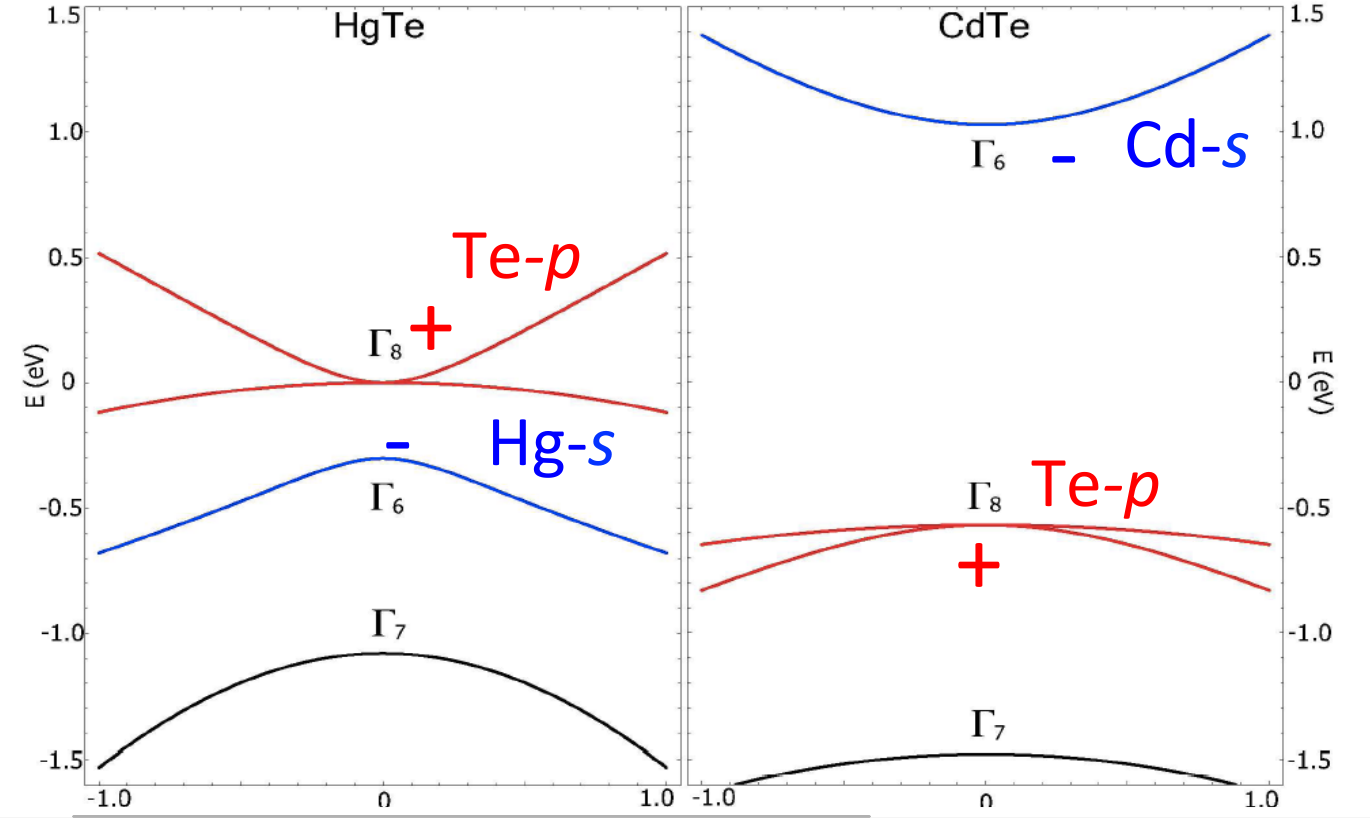
\includegraphics[height=2.4in,width=3.80in,viewport=0 5 1350 830,clip]{Figures/SOC_double-group_2.png}
%\caption{\tiny \textrm{Symmetry classification of the bands in the extended Kane model.}}%(与文献\cite{EPJB33-47_2003}图1对比)
\label{Fig:Relativistic-Effect}
\end{figure}
}

\section{旋转矩阵与旋-轨耦合项$\vec s\cdot\vec l$的计算}
\frame
{
	\frametitle{\textrm{Euler}角与旋转矩阵}
	从群论角度考虑,旋-轨耦合效应会引入双值群\textrm{(Double~group)}\footnote{\fontsize{5.2pt}{6.2pt}\selectfont{轨道角动量是三维空间的连续旋转本征值,可用\textrm{SO(3)}群表示;~自旋角动量则是二维复矢量的幺正群,用\textrm{SU(2)}群表示。两个群的\textrm{Lie}代数同构,但\textrm{Lie}群群元是一对二的关系。而点群都是\textrm{SO(3)}群的子群,因此不能用来描述\textrm{SU(2)}群,从而引入双值群}}

	双值群的生成元可以通过自旋轴向确定的\textrm{Euler}角确定。

	{\fontsize{6.5pt}{4.2pt}\selectfont{在旋-轨耦合计算时,通过指定磁化轴向,可确定\textrm{Euler}角}}
	\begin{figure}[h!]
\centering
\vspace*{-0.21in}
\hspace*{-0.1in}
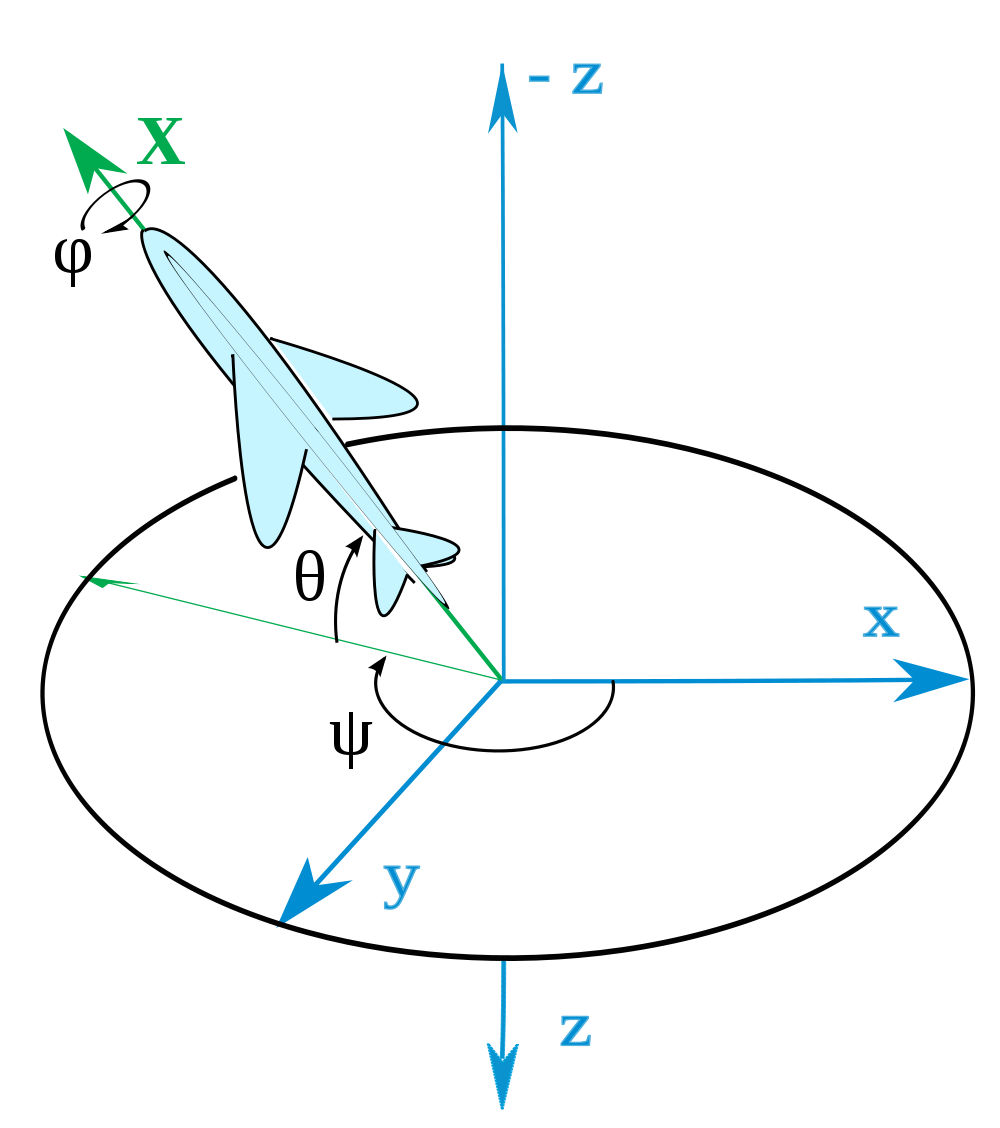
\includegraphics[height=1.7in,width=2.0in,viewport=2 5 1162 1180,clip]{Figures/euler-angles-yaw-aircraft-principal-axes-orientation-cartesian-coordinate-system.png}
\caption{\tiny \textrm{The Euler angles yaw aircraft-principal axes orientation Cartesian coordingate system.}}%(与文献\cite{EPJB33-47_2003}图1对比)
\label{Fig:Euler}
\end{figure}
}

\frame
{
	\frametitle{自旋翻转的\textrm{M\"obius}环示意}
	\begin{figure}[h!]
\centering
\vspace*{-0.10in}
%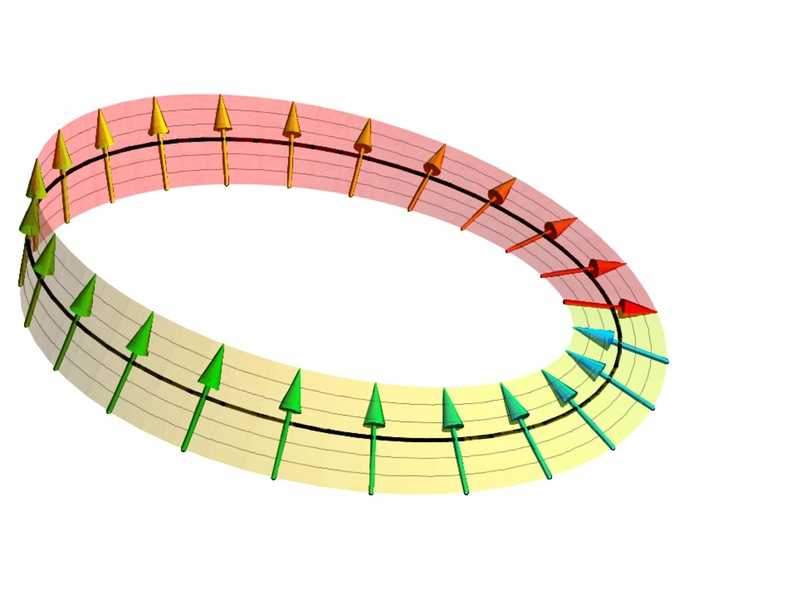
\includegraphics[height=2.5in,width=4.0in,viewport=0 30 330 250,clip]{Figures/spin_half_mobius.jpg}
%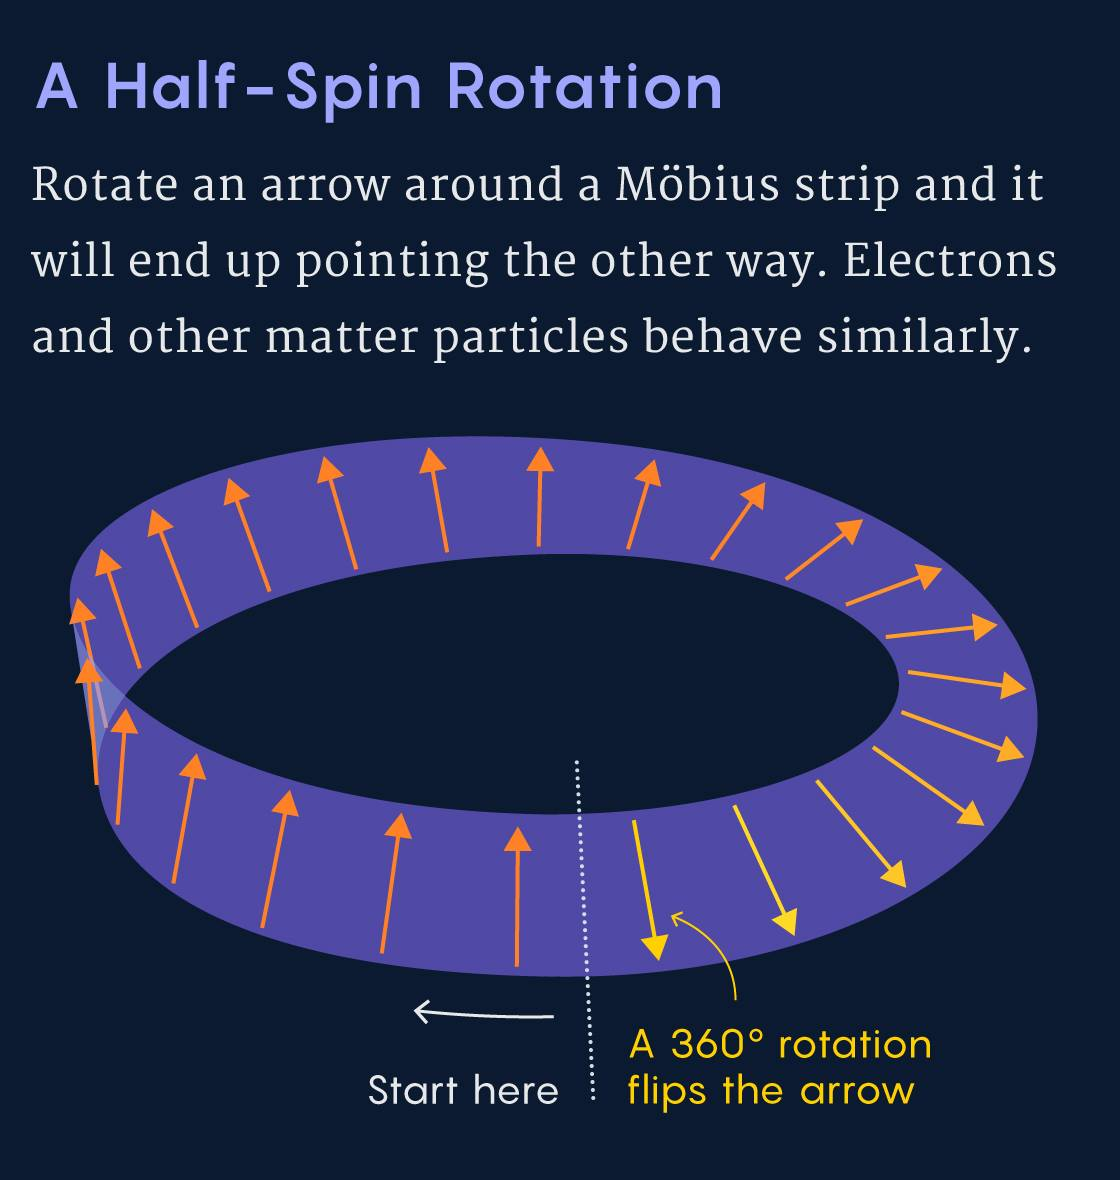
\includegraphics[height=2.5in,width=4.0in,viewport=0 30 1120 770,clip]{Figures/spin_half_mobius_2.jpg}
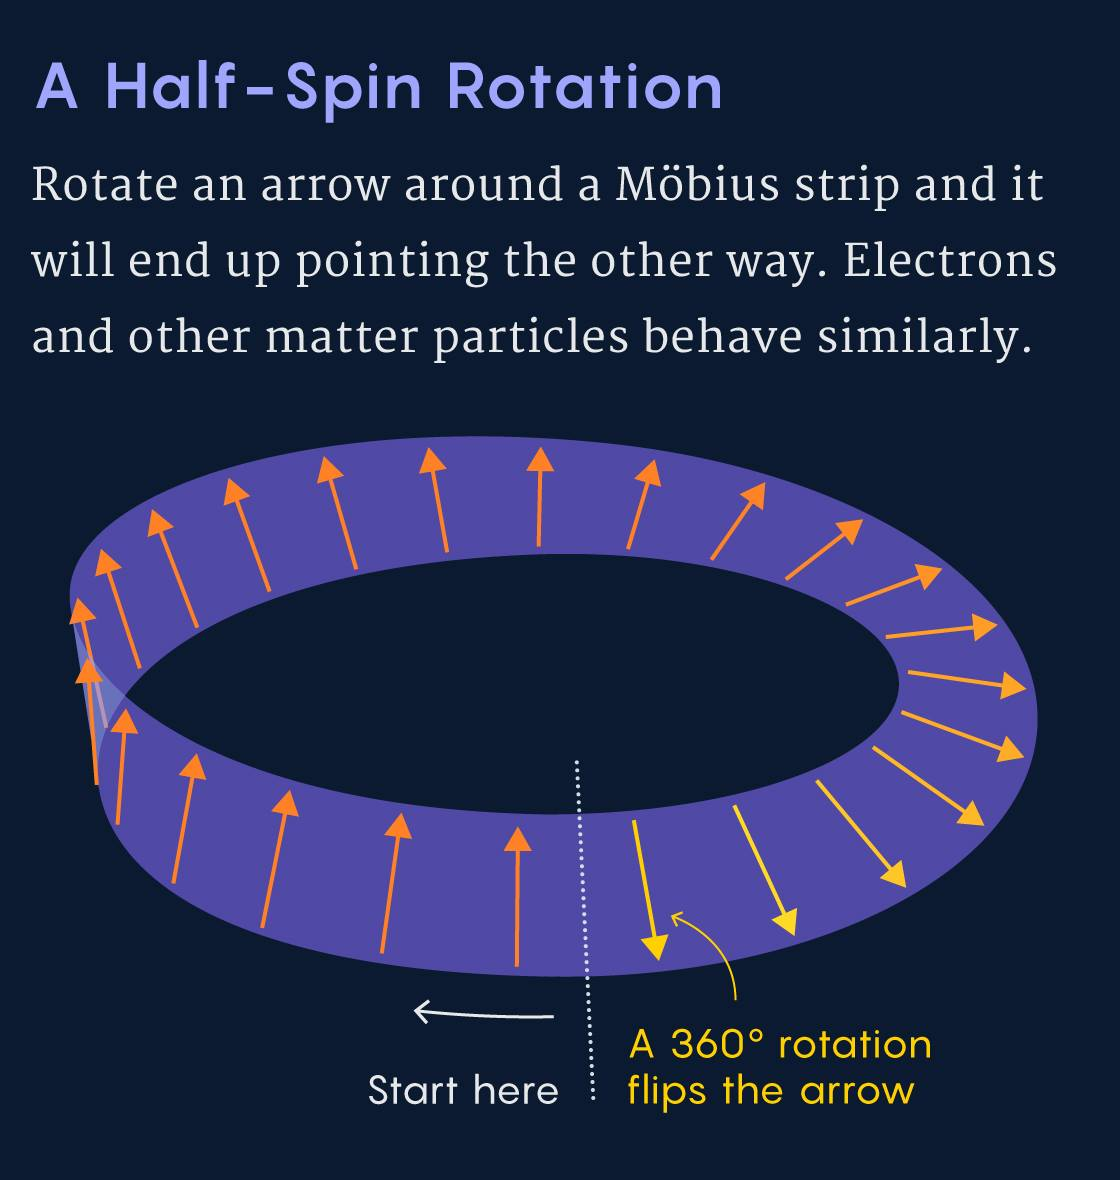
\includegraphics[height=2.7in,width=2.65in,viewport=0 0 1120 1170,clip]{Figures/spin_half_mobius_2.jpg}
\caption{\tiny \textrm{The geometrical representation of spinor follows the Mobius strip.}}%(与文献\cite{EPJB33-47_2003}图1对比)
\label{Fig:Mobius}
\end{figure}
}

\frame
{
	\frametitle{\textrm{Euler}角表示的旋转操作}
	{	\fontsize{6.5pt}{4.2pt}\selectfont{简要说明如下:
	旋-轨耦合引入\textrm{M\"obius}变换,用\textrm{Euler angles}表示为
	\begin{displaymath}
		\begin{aligned}
			\Pi_u(g_{\phi})=&\Pi_u\bigg[
				\begin{pmatrix}
					\cos\phi &-\sin\phi &0\\
					\sin\phi &\cos\phi &0\\
					0 &0 &1
				\end{pmatrix}
				\bigg]=&\pm
				\begin{pmatrix}
					\mathrm{e}^{\mathrm{i}\frac{\phi}{2}} &0\\
					0 &\mathrm{e}^{-\mathrm{i}\frac{\phi}{2}}
				\end{pmatrix}\\
			\Pi_u(g_{\theta})=&\Pi_u\bigg[
				\begin{pmatrix}
					1 &0 &0\\
					0 &\cos\theta &-\sin\theta\\
					0 &\sin\theta &\cos\theta
				\end{pmatrix}
				\bigg]=&\pm
				\begin{pmatrix}
					\cos\frac{\theta}{2} &\mathrm{i}\sin\frac{\theta}{2}\\
					\mathrm{i}\sin\frac{\theta}{2} &\cos\frac{\theta}{2}
				\end{pmatrix}
		\end{aligned}
	\end{displaymath}
	应用\textrm{Euler angles},可以定义旋转操作
\begin{displaymath}
		\begin{aligned}
			g(\phi,\theta,\psi)=g_{\phi}g_{\theta}g_{\psi}=
			\begin{pmatrix}
			%	\begin{aligned}
					\cos\phi &-\sin\phi &0\\
					\sin\phi &\cos\phi &0\\
					0 &0 &1
			%	\end{aligned}
			\end{pmatrix}
			\begin{pmatrix}
			%	\begin{aligned}
					1 &0 &0\\
					0 &\cos\theta &-\sin\theta\\
					0 &\sin\theta &\cos\theta
			%	\end{aligned}
			\end{pmatrix}
			\begin{pmatrix}
				\cos\psi &-\sin\psi &0\\
				\sin\psi &\cos\psi &0\\
				0 &0 &1
			\end{pmatrix}\\
			\begin{pmatrix}
				\cos\phi\cos\psi-\cos\theta\sin\phi\sin\psi &-\cos\phi\sin\psi-\cos\theta\sin\phi\cos\psi &\sin\phi\sin\theta\\
				\sin\phi\cos\psi+\cos\theta\cos\phi\sin\psi &-\sin\phi\sin\psi+\cos\theta\cos\phi\cos\psi &-\cos\phi\sin\theta\\
				\sin\psi\sin\theta &\cos\psi\sin\theta &\cos\theta
			\end{pmatrix}
		\end{aligned}
	\end{displaymath}
因此\textrm{SU(2)}群的生成元用\textrm{Euler}角表示
}}
}

\frame
{
	\frametitle{\textrm{Euler}表示的旋转操作}
	{	\fontsize{6.2pt}{4.2pt}\selectfont{
	\begin{displaymath}
		\begin{aligned}
			\Pi_u(g(\phi,\theta,\psi))=&\pm
			\begin{pmatrix}
				\mathrm{e}^{\mathrm{i}\frac{\phi}{2}} &0\\
				0 &\mathrm{e}^{-\mathrm{i}\frac{\phi}2}
			\end{pmatrix}
			\begin{pmatrix}
				\cos\frac{\theta}{2} &\mathrm{i}\sin\frac{\theta}{2}\\
				\mathrm{i}\sin\frac{\theta}{2} &\cos\frac{\theta}{2}
			\end{pmatrix}
			\begin{pmatrix}
				\mathrm{e}^{\mathrm{i}\frac{\psi}{2}} &0\\
				0 &\mathrm{e}^{-\mathrm{i}\frac{\psi}{2}}
			\end{pmatrix}\\
			=&\pm
			\begin{pmatrix}
				\cos\frac{\theta}{2}\mathrm{e}^{\mathrm{i}\frac{\phi+\psi}{2}} &\mathrm{i}\sin\frac{\theta}{2}\mathrm{e}^{\mathrm{i}\frac{\phi-\psi}{2}}\\
				\mathrm{i}\sin\frac{\theta}{2}\mathrm{e}^{-\mathrm{i}\frac{\phi-\psi}{2}} &\cos\frac{\theta}{2}\mathrm{e}^{-\mathrm{i}\frac{\phi+\psi}{2}}
			\end{pmatrix}
		\end{aligned}
	\end{displaymath}
为简化表示,习惯上将生成元记作
\begin{displaymath}
	\pm\Pi_u(g_{\alpha,\beta})=\pm
	\begin{pmatrix}
		\alpha &\beta\\
		-\overline{\beta} &\overline{\alpha}
	\end{pmatrix}
	\in\mathrm{SU(2)}
\end{displaymath}
不难看出有
\begin{displaymath}
	\begin{aligned}
		\cos\dfrac{\theta}{2}=|\alpha|,\qquad\qquad &\sin\dfrac{\theta}{2}=|\beta|, \qquad\qquad(0\leqslant\theta\leqslant\pi)\\
		\dfrac{\phi+\psi}{2}=\arg{\alpha},\qquad\qquad &\dfrac{\psi-\phi}{2}=\arg{\beta}
	\end{aligned}
\end{displaymath}
如果将$\Pi(g_{\alpha,\beta})$代入$\Pi_u(g(\phi,\theta,\psi))$则可将空间旋转操作$g(\phi,\theta,\psi)$用复数形式的$\alpha,\beta$表示为
\begin{displaymath}
	g_{\alpha,\beta}=
	\begin{pmatrix}
		\frac12\big(\alpha^2-\beta^2+\overline{\alpha^2}-\overline{\beta^2}\big) &\frac{\mathrm{i}}2\big(-\alpha^2-\beta^2+\overline{\alpha^2}+\overline{\beta^2}\big) &-\alpha\beta-\overline{\alpha}\overline{\beta}\\
		\frac{\mathrm{i}}2\big(\alpha^2-\beta^2-\overline{\alpha^2}+\overline{\beta^2}\big) &\frac12\big(\alpha^2+\beta^2+\overline{\alpha^2}+\overline{\beta^2}\big) &-\mathrm{i}\big(+\alpha\beta-\overline{\alpha}\overline{\beta}\big)\\
		\alpha\overline{\beta}+\overline{\alpha}\beta &\mathrm{i}\big(-\alpha\overline{\beta}+\overline{\alpha}\beta\big) &\alpha\overline{\alpha}-\beta\overline{\beta}
	\end{pmatrix}
\end{displaymath}
利用\textrm{Euler}角清楚地表明:~\textcolor{blue}{\textrm{SO(3)}与\textrm{SU(2)}构成满射同态群}
\begin{displaymath}
	\left\{
		\begin{aligned}
			p:~\mathrm{SU(2)}&\rightarrow \mathrm{SO(3)}\\
			\Pi_u(\pm g_{\alpha\beta})&\rightarrow g_{\alpha\beta}
		\end{aligned}
		\right.
\end{displaymath}
}}
}

\frame
{
	\frametitle{能带的双值群表示}
	锌残杂的半导体\textrm{Si},\textrm{Ge},\textrm{GaAs},\textrm{CdTe},\textrm{HgTe}的能带
	\begin{figure}[h!]
\centering
\vspace*{-0.10in}
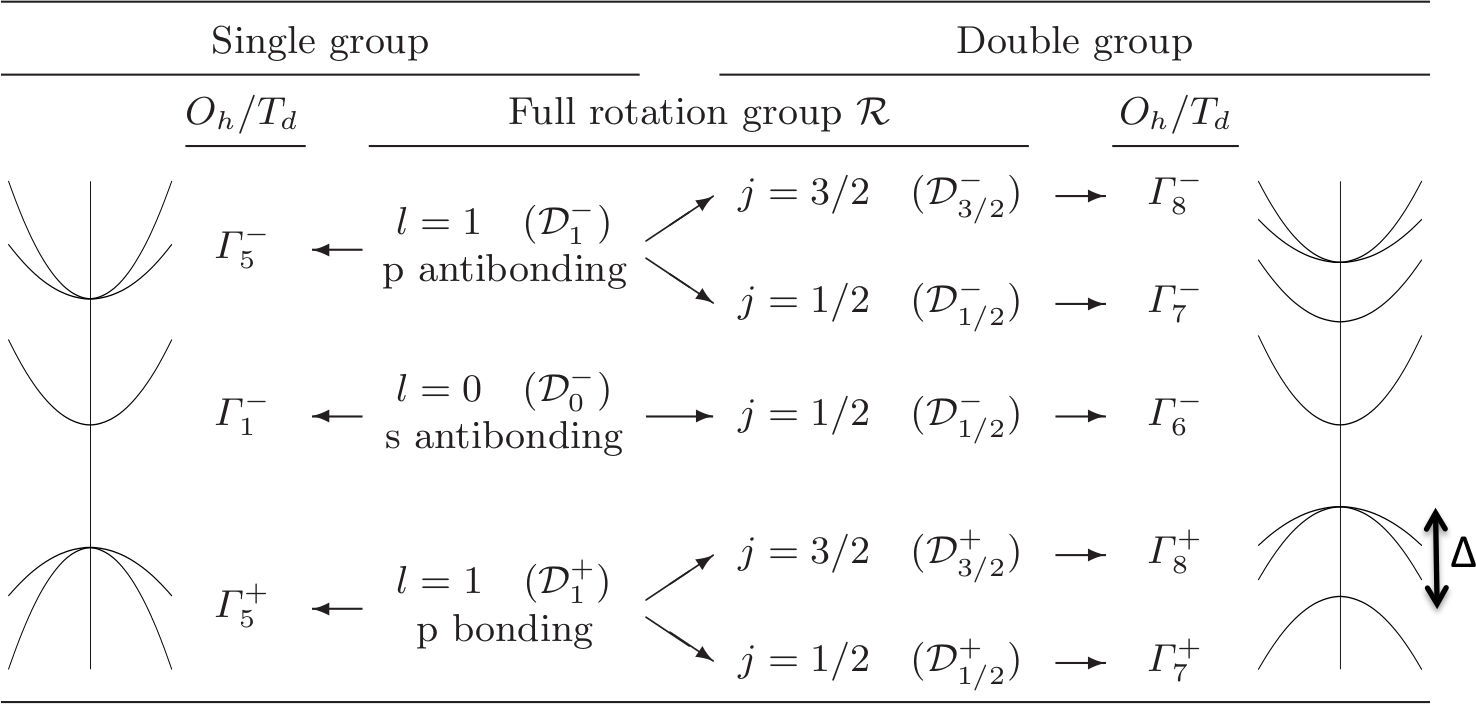
\includegraphics[height=2.1in,width=4.00in,viewport=0 0 1490 730,clip]{Figures/SOC_double-group.png}
\caption{\tiny \textrm{Symmetry classification of the bands in the extended Kane model.}}%(与文献\cite{EPJB33-47_2003}图1对比)
\label{Fig:Double-Group}
\end{figure}
}

\frame
{
	\frametitle{旋-轨耦合项的贡献}
	考虑旋-轨耦合后\textrm{Hamiltonian}的修正为
	\begin{displaymath}
		H_{\mathrm{SO}}=\dfrac{h}{2Mc^2}\dfrac1{r}\dfrac{\mathrm{d}V}{\mathrm{d}r}\vec{s}\cdot\vec{l}
	\end{displaymath}
%	随着磁化轴向的确定,空间\textrm{Euler}角确定,\textrm{Euler}角表示的矩阵$\Pi_u$表示局域旋转矩阵影响,具体到$\vec\sigma\cdot\vec l$项

%	对于给定的角动量$l$,
	算符$\vec{s}\cdot\vec{l}$主要作用于波函数的角度和自旋部分,即
\begin{displaymath}
	\mathrm{SO}_{m_1,m_2,\sigma_1,\sigma_2,L}=\langle\sigma_1|\langle y_{l,m_1}|\hat S\cdot\hat L|y_{l,m_2}\rangle|\sigma_2\rangle=\langle\sigma_1|\hat S|\sigma_2\rangle\langle y_{l,m_1}|\hat L|y_{l,m_2}\rangle
\end{displaymath}

因此可分别计算$\langle y_{l,m_1}|\hat l|y_{l,m_2}\rangle$和$\langle\sigma_1|\hat s|\sigma_2\rangle$:

利用升降算符与复数表示的球谐函数的关系
	{	\fontsize{8.2pt}{4.2pt}\selectfont{
\begin{displaymath}
	\begin{aligned}
		\hat{L}_-y_{l,m}=&\hbar\sqrt{l(l+1)-m(m-1)}y_{l,m-1}=&\hbar\sqrt{(l+m)(l-m+1)}y_{l,m-1}\\
		\hat{L}_+y_{l,m}=&\hbar\sqrt{l(l+1)-m(m+1)}y_{l,m+1}=&\hbar\sqrt{(l-m)(l+m+1)}y_{l,m+1}
	\end{aligned}
\end{displaymath}}}
这里$y_{l,m}$表示复数表示的球谐函数。

%电子自旋算符表示分为$|\alpha\rangle=\dfrac12\sigma$和$|\beta\rangle=-\dfrac12\sigma$%,当电子自旋与$z$方向平行时,$\mathbf{l}\cdot\mathbf{s}$将分解为
}

\frame
{
	\frametitle{旋-轨耦合项的贡献}
类似地,自旋角动量的升降算符为
\begin{displaymath}
	\begin{aligned}
		\hat S_-=&\hat S_x-\mathrm{i}\hat S_y\\
		\hat S_+=&\hat S_x+\mathrm{i}\hat S_y
	\end{aligned}
\end{displaymath}
因此直角坐标系下的自旋算符用升降算符表示为
\begin{displaymath}
	\begin{aligned}
		\hat S_x=&\dfrac12(\hat S_++\hat S_-)\\
		\hat S_y=&\dfrac1{2\mathrm{i}}(\hat S_+-\hat S_-)
	\end{aligned}
\end{displaymath}

根据上述讨论,$\vec{s}\cdot\vec{l}$可表示为:
\begin{displaymath}
%	\mathbf{l}\cdot\mathbf{s}_{\mathrm{orig}}=
	\begin{pmatrix}
		\langle\alpha|\mathrm{SO}|\alpha\rangle &\langle\alpha|\mathrm{SO}|\beta\rangle \\
		\langle\beta|\mathrm{SO}|\alpha\rangle &\langle\beta|\mathrm{SO}|\beta\rangle
	\end{pmatrix}
\end{displaymath}
这里$\mathrm{SO}$略去角动量下标,表示将$\vec s\cdot\vec l$展开后的形式
}

\frame
{
	\frametitle{旋-轨耦合项的贡献}
根据升降算符的关系,不难看出,$\vec{s}\cdot\vec{l}$的矩阵表示中
\begin{enumerate}
	\item \textcolor{blue}{电子自旋$z$方向分量,对矩阵的对角元有贡献}
	\item \textcolor{magenta}{电子自旋在$x$与$y$方向分量,将对矩阵的非对角元有贡献}
\end{enumerate}

自旋角动量是二维复矢量的幺正群,用\textrm{SU(2)}群表示,指定磁化轴向后,\textrm{SU(2)}群的生成元可由\textrm{Euler}角表示的旋转矩阵$\Pi_u$表示,
\begin{displaymath}
	\vec{s}\cdot\vec{l}= \Pi_u^{\ast}\textcolor{red}{\vec{s}\cdot\vec{l}_{\mathrm{orig}}}\Pi_u
\end{displaymath}
	{\fontsize{6.2pt}{4.2pt}\selectfont{
具体地,针对各类$l$和$s$的组合,$\vec s\cdot\vec l$矩阵的形式有(单位是$\hbar^2$)
		\begin{itemize}
			\item $\Delta m_s=0$~\&~$\Delta m =0$,矩阵对角元有贡献项,形如
	\begin{displaymath}
			\Pi_u^{\ast} 
			\begin{pmatrix}
				\dfrac{m_l}2 &0\\
				0 &\dfrac{m_l}2
			\end{pmatrix}
			\Pi_u
	\end{displaymath}
\item $|\Delta m_s|=1$~\&~$|\Delta m|=1$,矩阵非对角元有贡献项,形如
	\begin{displaymath}
		\begin{aligned}
			\Pi_u^{\ast}
			\begin{pmatrix}
			0	&\frac{\sqrt{(l+m_l)(l-m_l+1)}}2\\
			0 &0
			\end{pmatrix}
			\Pi_u\qquad\mbox{和}\qquad
			\Pi_u^{\ast} 
			\begin{pmatrix}
				0 &0\\
				\frac{\sqrt{(l-m_l)(l+m_l+1)}}2 &0
			\end{pmatrix}
			 \Pi_u
		\end{aligned}
	\end{displaymath}
		\end{itemize}
具体可根据$l,m_l,s,m_s$允许的组合依次类推
}}
}

\subsection{旋-轨耦合与二次变分}
\frame
{
	\frametitle{旋-轨耦合作用大小的估计}
\begin{figure}[h!]
\centering
\vspace*{-0.10in}
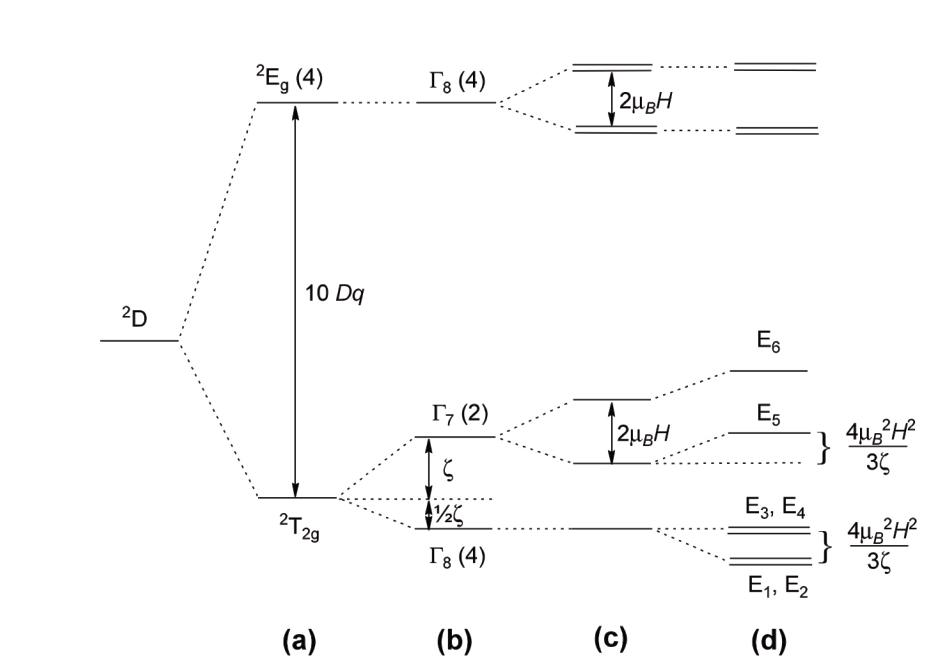
\includegraphics[height=2.40in,width=3.71in,viewport=80 0 930 620,clip]{Figures/Crystal_Field-SOC-magnetism.png}
\caption{\fontsize{6.2pt}{4.2pt}\selectfont{\textrm{The diagram is for a $d^1$ octahedral complex under a magnetic field: (a)~ligand field splitting, (b)~spin-orbit coupling, (3)~first-order Zeeman splitting, (d)~second-order Zeeman splitting.}}}%(与文献\cite{EPJB33-47_2003}图1对比)
\label{Crystal-Field_SOC-magnetism}
\end{figure}
}

\frame
{
	\frametitle{标量相对论计算与自旋极化}
	用旋-轨耦合处理价电子体系,先求解自旋分离的标量相对论波函数$\tilde{g}(r)$和$\tilde{f}(r)$
	\begin{displaymath}
		\begin{aligned}
			&-\frac{\hbar^2}{2Mr^2}\frac{\mathrm{d}}{\mathrm{d}r}\left[ r^2\frac{\mathrm{d}\tilde{g}(r)}{\mathrm{d}r} \right]+\left[ V(r)+\frac{\hbar^2}{2Mr^2}\frac{l(l+1)}{r^2} \right]\tilde{g}(r)\\
			&-\frac{\hbar^2}{4M^2c^2}\frac{\mathrm{d}V(r)}{\mathrm{d}r}\frac{\mathrm{d}\tilde{g}(r)}{\mathrm{d}r}=\varepsilon\tilde{g}(r)\\
			&\tilde{f}(r)=\frac{h}{2Mc}\frac{\mathrm{d}\tilde{g}(r)}{\mathrm{d}r}\\
		\end{aligned}
	\end{displaymath}
	由于在标量相对论近似下,自旋是好的量子数,因此可分别组合到\textcolor{blue}{自旋波函数}
	\begin{displaymath}
		\phi_{lm}^{\uparrow}=\left( 
		\begin{matrix}
			\tilde{g}_l^{\uparrow}Y_{lm}\\
			-\mathrm{i}\tilde{f}_l^{\uparrow}Y_{lm}
		\end{matrix}
		\right)\chi_{\uparrow}\quad
		\phi_{lm}^{\downarrow}=\left( 
		\begin{matrix}
			\tilde{g}_l^{\downarrow}Y_{lm}\\
			-\mathrm{i}\tilde{f}_l^{\downarrow}Y_{lm}
		\end{matrix}
		\right)\chi_{\downarrow}\quad
		\chi_{\uparrow}=\left( 
		\begin{matrix}
			1\\
			0
		\end{matrix}
		\right)\quad
		\chi_{\downarrow}=\left( 
		\begin{matrix}
			0\\
			1
		\end{matrix}
		\right)
	\end{displaymath}
}

\frame
{
	\frametitle{旋-轨耦合与二次变分}
	\begin{itemize}
		\setlength{\itemsep}{20pt}
		\item \textcolor{blue}{旋-轨耦合作用于标量相对论的大分量$\tilde{g}_l$,因此对自旋向上和向下部分都有贡献}
		\item 在原有\textrm{Hamiltonian}基础上直接引入旋-轨耦合算符$H_{\mathrm{SO}}$,将使基函数加大一倍(\textrm{spin-up+spin-dn})\\
			不适应大的计算体系
		\item \textcolor{red}{二次变分}
	\begin{displaymath}
		\left[ 
			\begin{matrix}
				\ddots & & &\raisebox{-1.0ex}[0pt]{\Huge0}  \\
				&\mathbf{H}_{\mathrm{SO}}^{\alpha\alpha} &\mathbf{H}_{\mathrm{SO}}^{\alpha\beta} &\\
			&\mathbf{H}_{\mathrm{SO}}^{\beta\alpha} &\mathbf{H}_{\mathrm{SO}}^{\beta\beta} &\\
			\raisebox{0.8ex}[0pt]{\Huge0} & & & \ddots
			\end{matrix}
			\right]
	\end{displaymath}
	\end{itemize}
}

\frame
{
	\frametitle{旋-轨耦合与二次变分}
	\begin{itemize}
		\item \textcolor{red}{二次变分的实现}
			\begin{enumerate}
				\setlength{\itemsep}{30pt}
				\item \textcolor{brown}{正常求解自旋极化本征态波函数(不含$H_{\mathrm{SO}}$)得
%					\begin{displaymath}
						$\psi_n^{\uparrow}\quad\varepsilon_n^{\uparrow}\quad\psi_n^{\downarrow}\quad\varepsilon_n^{\downarrow}$
%					\end{displaymath}
					}
				\item \textcolor{brown}{用自旋极化本征态波函数为基函数,对总\textrm{Hamiltonian}\\(包含$H_{\mathrm{SO}}$)构造矩阵更方便:}\\
					\textcolor{red}{矩阵维度低且近似对角化,对角元是标量相对论本征值\\大多数情况下,$H_{\mathrm{SO}}$比较小,计算方便}
				\item \textcolor{brown}{二次变分增加了变分自由度}
			\end{enumerate}
	\end{itemize}
}

\frame
{
	\frametitle{\textrm{LAPW~}框架下处理旋-轨耦合}
\begin{figure}[h!]
\centering
\vspace*{-0.10in}
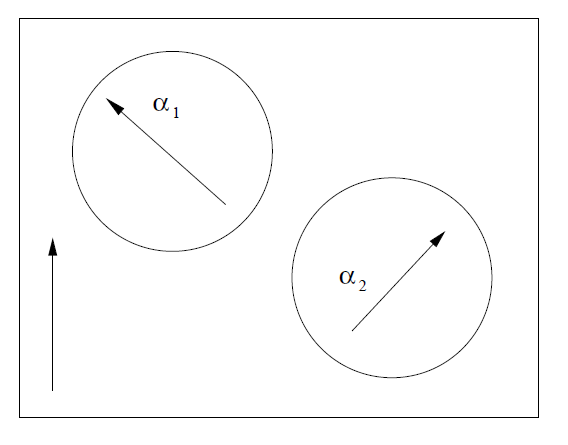
\includegraphics[height=1.45in,width=2.01in,viewport=0 10 430 330,clip]{Figures/WIENNCM_Sphere.png}
\caption{\small \textrm{The spin coordinate frmaes.}}%(与文献\cite{EPJB33-47_2003}图1对比)
\label{WIENNCM_sphere}
\end{figure}
考虑旋-轨耦合后,\textrm{LAPW~}基函数表示为
\begin{displaymath}
	\footnotesize\hskip -50pt \varphi^{\vec G}_{\sigma}=\left\{
  \begin{aligned}
	  &\mathrm{e}^{\mathrm{i}(\vec G+\vec k)\cdot\vec r}\chi_{\sigma}\\
	  &\sum_{\sigma^{\alpha}}\sum_{lm}[A^{\vec G_{\sigma\sigma^{\alpha}}}_{lm}u_l^{\sigma^{\alpha}}+B^{\vec G_{\sigma\sigma^{\alpha}}}_{lm}\dot u_l^{\sigma^{\alpha}}]Y_{lm}\chi_{\sigma^{\alpha}}
  \end{aligned}
\right.
\end{displaymath}
}

\frame
{
	\frametitle{\textrm{LAPW~}框架下处理旋-轨耦合}
\begin{figure}[h!]
\centering
\vspace*{-0.10in}
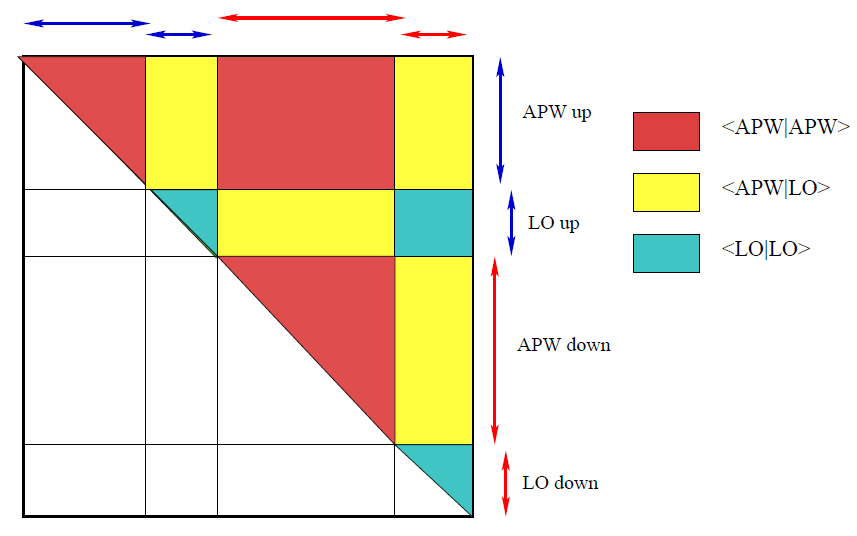
\includegraphics[height=2.19in,width=3.15in,viewport=0 0 650 430,clip]{Figures/WIENNCM_Ham.png}
\caption{\small \textrm{Allocation of the Hamiltonian and overlap matrix.}}%(与文献\cite{EPJB33-47_2003}图1对比)
\label{WIENNCM_Ham}
\end{figure}
}

\section{固体中的旋-轨耦合}
\frame
{
	\frametitle{固体材料中的两类旋-轨耦合}
	\begin{itemize}
		\item \textcolor{blue}{对称性无关的旋-轨耦合}\\
			存在于各类晶体中:\\
			源于原子轨道本身的旋-轨耦合
		\item \textcolor{blue}{对称性相关的旋-轨耦合}\\
			\begin{enumerate}
		\setlength{\itemsep}{5pt}
				\item 存在于表面和体相的广义的旋-轨耦合:\\
					局域空间非对称\textrm{(Local-Space-Asymmetry, LSA)}\\
				\item 存在于没有倒反对称性\textrm{(inversion~symmetry)}的晶体中:\\
			表面:~\textrm{Bychkov-Rashba}效应:\\
			表面诱导的非对称\textrm{(Surface-Induced-Asymmetry, SIA)}\\
			\vskip 4pt
			体相:~\textrm{Dresselhaus}相互作用:\\
			体相诱导的非对称\textrm{(Bulk-Induced-Asymmetry, BIA)}\\
			\end{enumerate}
	\end{itemize}
}

\frame
{
	\frametitle{时间反演与倒反对称性}
	\begin{itemize}
		\item 时间反演对称\textrm{(Time-reversal symmetry, TRS)}\\
			\begin{displaymath}
			\left.
				\begin{aligned}
					\vec s&\rightarrow -\vec s\\
					\vec l&\rightarrow -\vec l\\
					\vec s\cdot\vec l&\rightarrow \vec s\cdot\vec l\\
					\vec k&\rightarrow-\vec k
				\end{aligned}\right\}\Longrightarrow E_n(\vec s,\vec k)=E_n(-\vec s,-\vec k)
			\end{displaymath}
		\item 倒反对称\textrm{(Inversion symmetry, IS)}
			\begin{displaymath}
			\left.
				\begin{aligned}
					\vec s&\rightarrow \vec s\\
					\vec l&\rightarrow \vec l\\
					\vec s\cdot\vec l&\rightarrow \vec s\cdot\vec l\\
					\vec k&\rightarrow-\vec k
				\end{aligned}\right\}\Longrightarrow E_n(\vec s,\vec k)=E_n(\vec s,-\vec k)
			\end{displaymath}
	\end{itemize}
}

\frame
{
	\frametitle{时间反演-倒反对称破缺与能带}
	\begin{itemize}
		\item 时间反演-倒反对称性
\begin{figure}[h!]
\centering
\vspace*{-0.15in}
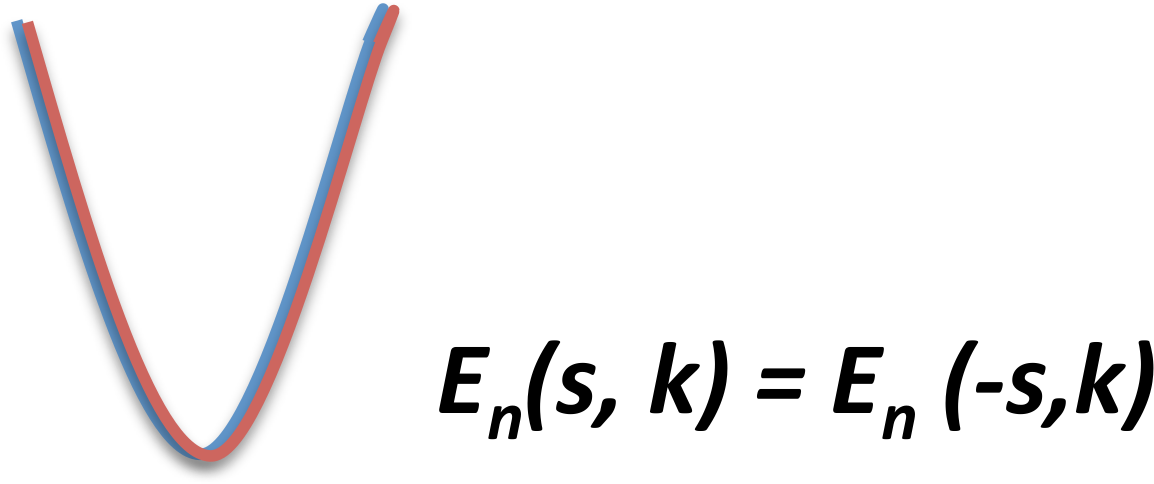
\includegraphics[height=1.25in,width=2.90in,viewport=0 0 1155 530,clip]{Figures/SOC_TRS-IS.png}
%\caption{\small \textrm{Allocation of the Hamiltonian and overlap matrix.}}%(与文献\cite{EPJB33-47_2003}图1对比)
\label{Symmetry-TRS-IS}
\end{figure}
\item 时间反演-倒反对称破缺
\begin{figure}[h!]
\centering
\vspace*{-0.15in}
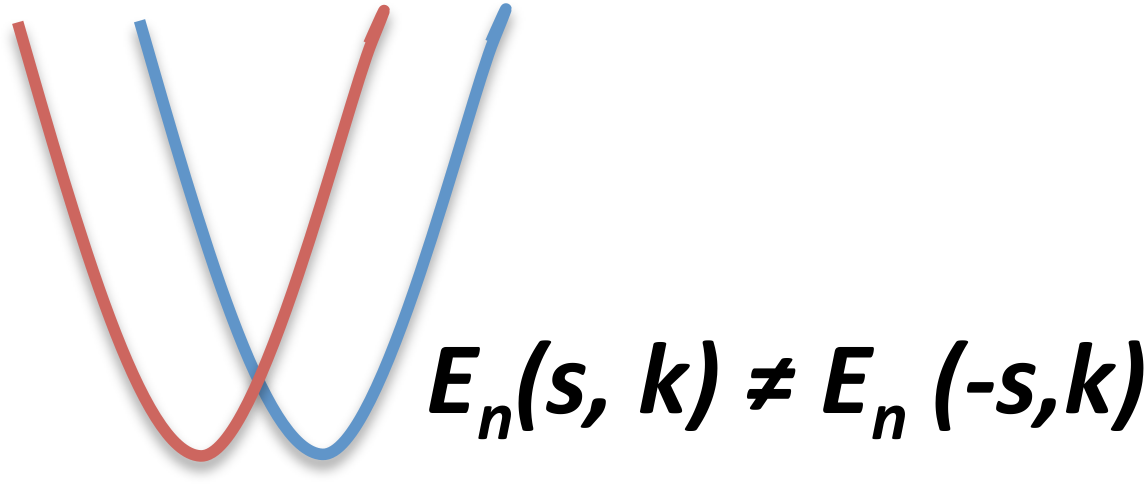
\includegraphics[height=1.25in,width=2.90in,viewport=0 0 1155 530,clip]{Figures/SOC_TRS-IS_breaking.png}
%\caption{\small \textrm{Allocation of the Hamiltonian and overlap matrix.}}%(与文献\cite{EPJB33-47_2003}图1对比)
\label{Symmetry-TRS-IS-breaking}
\end{figure}
	\end{itemize}
}

\frame
{
	\frametitle{\textrm{Rashba}效应}
	\textrm{Rashba}效应:~界面电场诱导的对称性破缺
\begin{figure}[h!]
\centering
\vspace*{+0.05in}
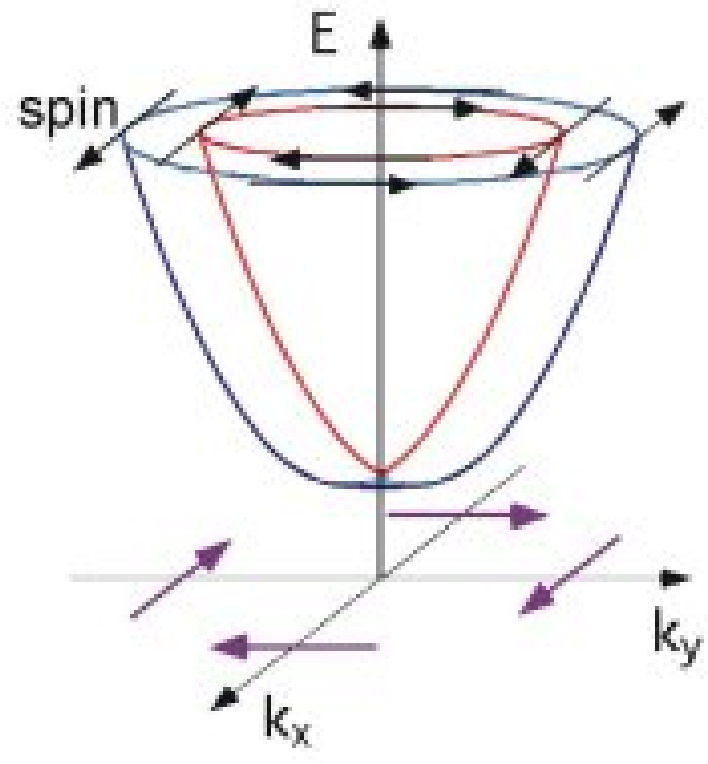
\includegraphics[height=1.25in,width=1.20in,viewport=0 0 700 760,clip]{Figures/SOC_Rashba_effect.png}
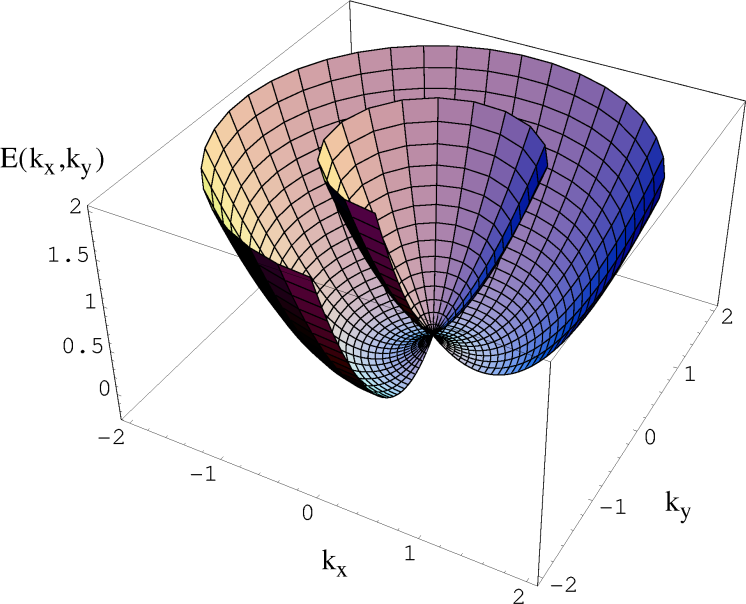
\includegraphics[height=1.25in,width=1.40in,viewport=0 0 750 600,clip]{Figures/SOC_Rashba-1.png}
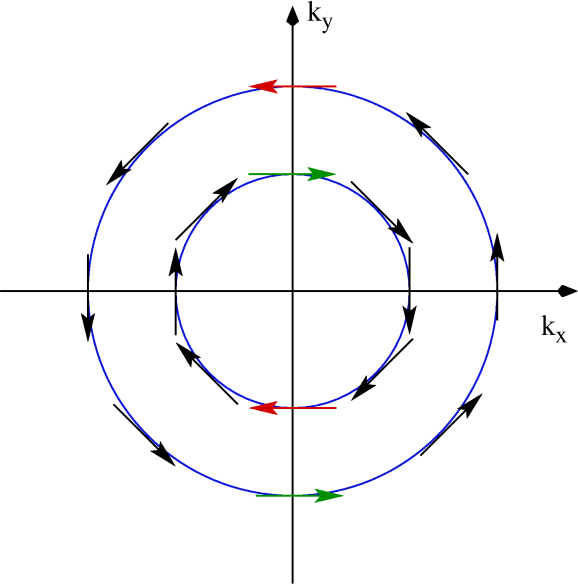
\includegraphics[height=1.25in,width=1.30in,viewport=0 0 650 590,clip]{Figures/SOC_Rashba-2.png}
%\caption{\small \textrm{Allocation of the Hamiltonian and overlap matrix.}}%(与文献\cite{EPJB33-47_2003}图1对比)
\label{Rashba_effect}
\end{figure}

	\begin{itemize}
	\item \textrm{Rashba~Hamiltonian}起源:~界面产生的电场$\mathbf E~(\mathbf E\parallel \hat z)$%引起的旋-轨耦合的形式为
		\begin{displaymath}
			\vec H_{\mathrm{Rashba}}=\alpha(\vec\sigma\times\vec p)\cdot\hat z
		\end{displaymath}
		其中:~$\alpha$是\textrm{Rashba}耦合系数 $\alpha=\dfrac{g\mu_BE_z}{2mc^2}$\\
		$\vec p$是电子的动量\\
		$\sigma$是自旋(\textrm{Pauli}矩阵中的矢量)
	\end{itemize}
}

\frame
{
	\frametitle{\textrm{Rashba}效应}
	\begin{itemize}
	\item \textrm{Rashba}效应描述的是动量相关的表面态二维自旋能带裂分,源于
		\begin{enumerate}
			\item 沿$\hat z$向(垂直于二维平面)的势倒反对称性破缺时,形成的电场
				\begin{displaymath}
					\mathbf E=E_z\hat z=-\dfrac1{e}\nabla V
				\end{displaymath}
			\item 旋-轨耦合
				\begin{displaymath}
					\begin{aligned}
						\mathbf B=&\dfrac1{c^2}\mathbf{E}\times\vec v\\
						\vec H_{\mathrm{SO}}=&\dfrac{g\mu_B}{2c^2}(\vec v\times\mathbf E)\cdot\sigma
					\end{aligned}
				\end{displaymath}
		\end{enumerate}
	\end{itemize}
}
